\chapter{Conclusion}
\chaptermark{Conclusion}
\cleardoublepage

\minitoc

\section{Overview of the thesis}
\begin{refsection}


  Three key points had been identified: number of primary particles, distortion effects of the profile, the choice of the reading system. 
  
  The conditions at ESS are particularly unfavourable for the ionization cross sections and the high vacuum in the accelerator does not work in our favour. Calculations (Bethe and PAI) and simulations show that the order of magnitude of the number of primary particles is about a few thousand particles per pulse beam under nominal ESS conditions. This number seems sufficient to carry out a measurement assuming that tey are correctly detected.

  Non-uniformity of the electric field can be effectively corrected using field correctors and separation discs regardless of the power supply configuration used. However, the symmetrical mode is easier to correct and reduces the maximum voltage required.
  Simulations clearly show that ions are less sensitive to the space charge effect and initial velocity of particle. Measurement with electrons introduces an error that does not allow the ESS requirements to be met. It is impossible to install a corrector magnet to constrain the electron trajectories. Therefore, the profile measurement will be done with ions.

  The use of ions makes the choice of the readout a more complicated. Strips are an robust method but require enough sensitive and low-noise electronics to be able to detect such low charge quantities.
  The MCPs amplifies the signal but these devices tend to age. Silicon detectors are very promising because they are very sensitive, resistant and fast. However, the detection of low energetic ions is not ensured and the implementation is quite complex. 

  In this thesis

  \section{Final design and outlooks}


  During the tests done at IPHI, we used a simple CF200 flange to support the IPM (Fig. \ref{fig:bride_simple}). 
  For the manufacturing of the IPM, we thought that 2 independent flanges CF200 and CF160 (Fig. \ref{fig:bride_double}) will ease the assembling process and also the maintenance. This later configuration presents the following advantages. 
  
  \begin{figure}[!ht]
	\begin{subfigure}[t]{0.25\textwidth}
		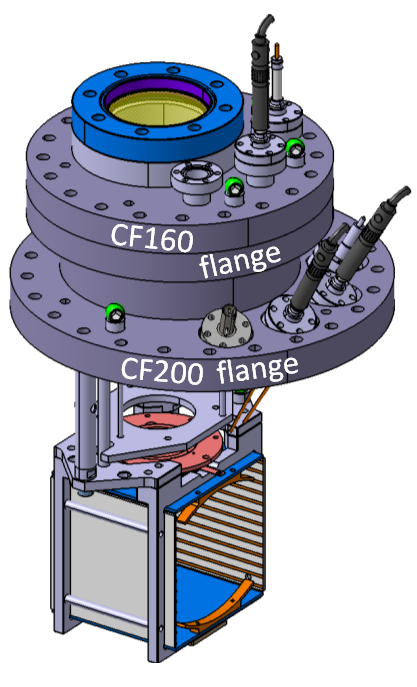
\includegraphics[width=\textwidth]{05_Conclusion/figures/fig000_bride_double2_a}
		\caption{A 3D drawing of the new design.}
		\label{}
	\end{subfigure}
	~
	\begin{subfigure}[t]{0.75\textwidth}
		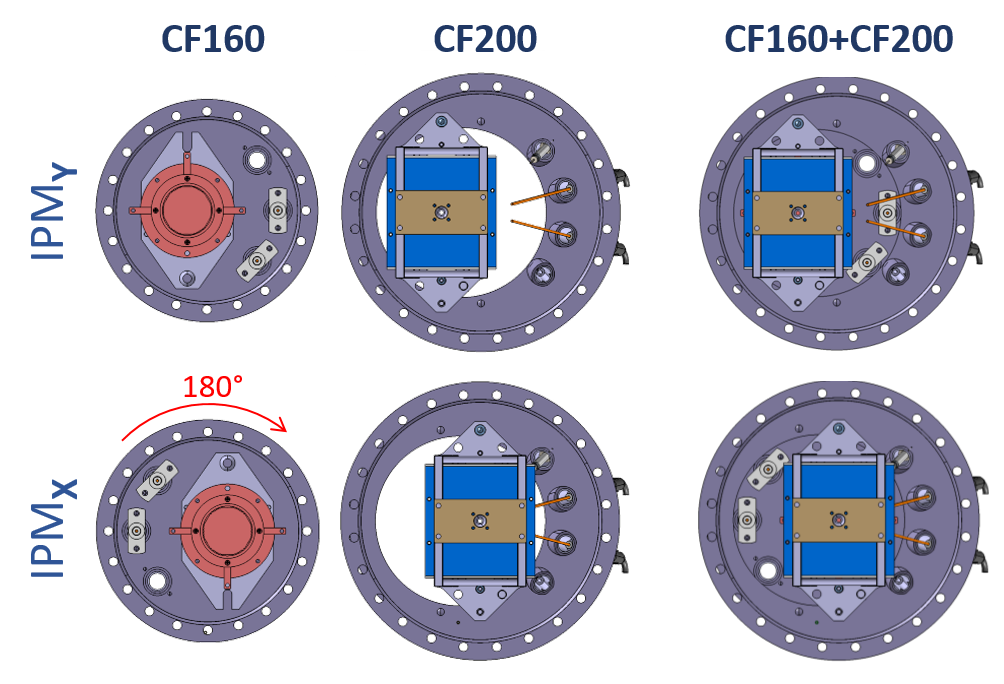
\includegraphics[width=\textwidth]{05_Conclusion/figures/fig000_bride_double2_b}
		\caption{The new design allow to remove MCP easily and is independent to the IPM direction.}
		\label{}
	\end{subfigure}
	\caption[The new IPM design]{The new IPM design \cite{JacquesCDR2019}.}
	\label{chap5:fig:bride_double}
\end{figure}

  Once the complete IPM set is mounted on the LWU VC, alignment can be done by measuring all sight pods on the CF200. Then, if MCP has to be removed (unscrew the CF160), the IPM cage linked to the CF200 stays fixed. MCP can be changed but, no alignment are necessary. We just have to measure with the CMOS camera the 4 crosses which will be engraved on the electrode plate back. This new configuration is compliant with a better reliability of the IPM since the MCP change may be done quickly, with no impact on alignment. Furthermore, the CF160 flange with its MCP bracket, HV viewports is quite light and can be easily operated.
  
  For assembling the whole IPM, it is more convenient to prepare first the CF200 and all its belonging items, and then the CF160 ones. It allows minimizing the MCP in oxygen atmosphere.
  
  Furthermore, the set made of CF160 and pMCP holder is light with a small lever arm easy to manipulate.
  
  The IPMs X and Y are similar: while X is centered on the CF200 LWU viewport, Y is shifted by 36 mm to its CF200 axis. The trick for mounting both IPMs, is to rotate the CF160 by 180° wrt the CF200 flange. This is of great interest for manufacturing purpose.

  In the case where the radiation background should shorten the MCP lifetime down to a year, it would be necessary to set a camera at remote distance in a shielded area. Two solutions are investigated to transport the image over up to 10\,m, where the camera can be shielded in the bottom of the nearby Stub. The solution to get a camera detecting single events, i.e. an ion hitting the MCP is been studied at ESS. The document presents two alternative imaging systems: the first one using a fiberscope and lenses is sketched on Fig. \ref{fig:fiberscope}, while the other one based on 2 mirrors and an objective lens can be seen on Fig. \ref{fig:miror}. 

  \begin{figure}[!ht]
	\begin{subfigure}[t]{0.5\textwidth}
		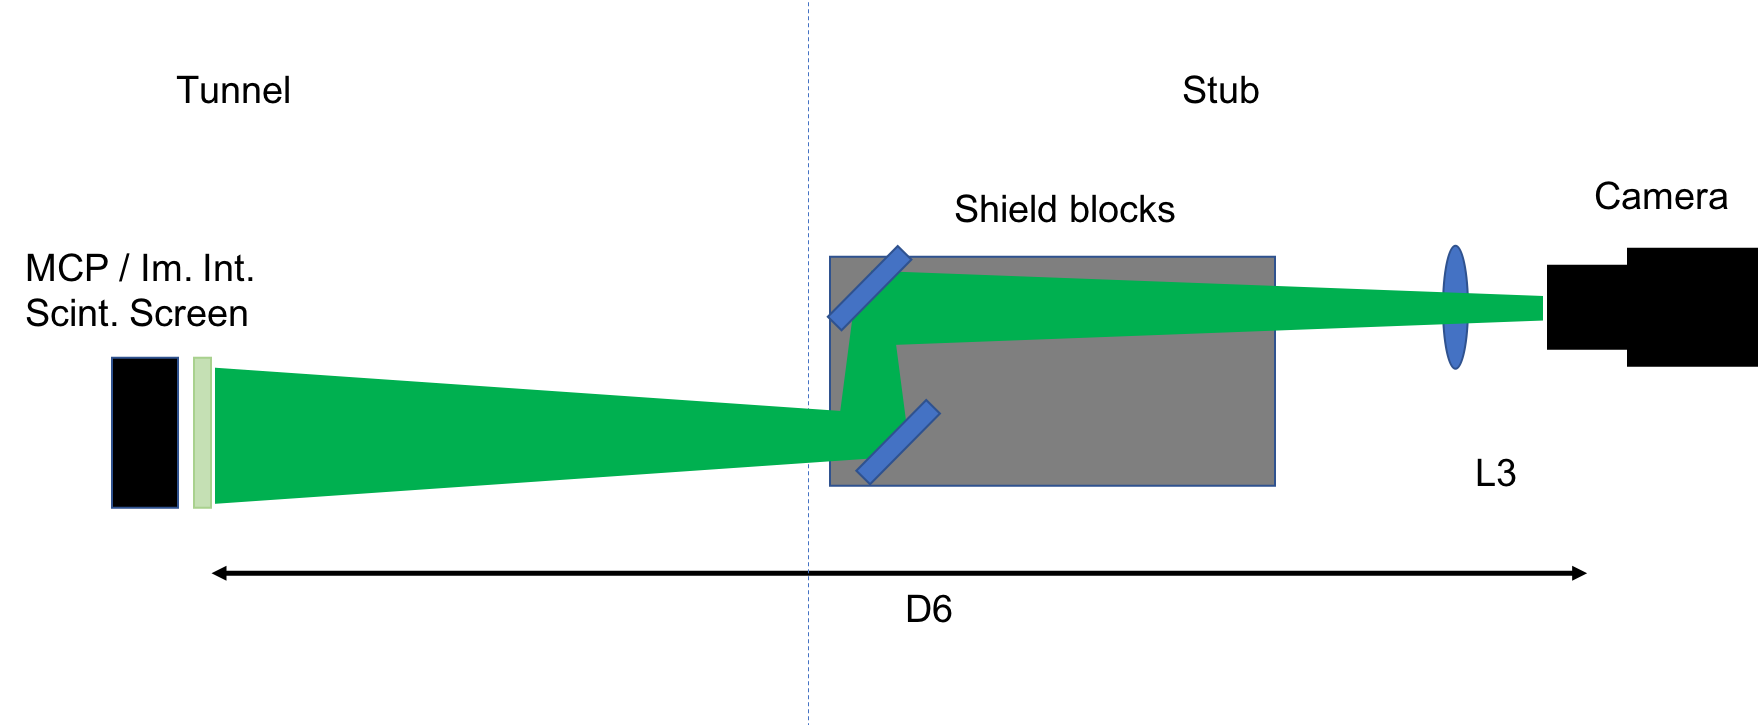
\includegraphics[width=\textwidth]{05_Conclusion/figures/fig000_schematic_telescop_lens}
		\caption{}
		\label{}
	\end{subfigure}
	~
	\begin{subfigure}[t]{0.5\textwidth}
		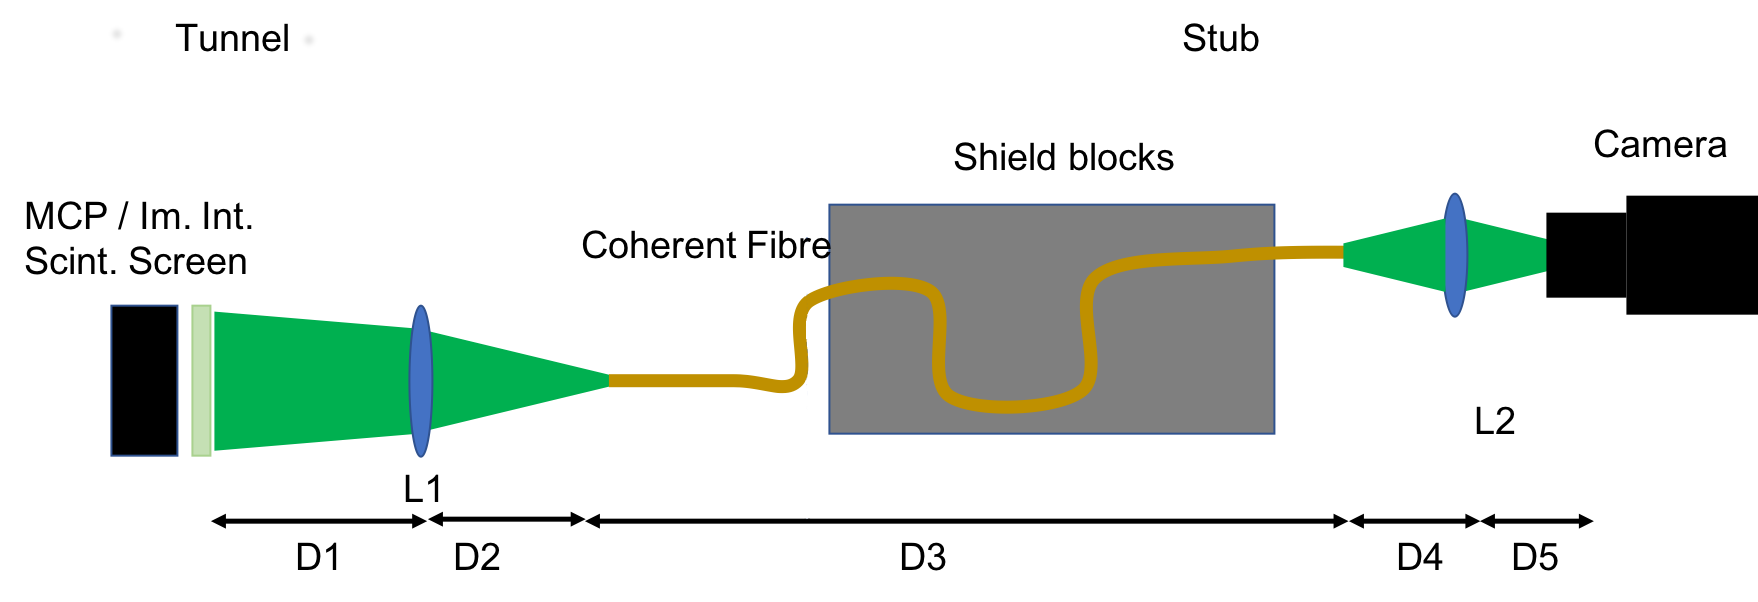
\includegraphics[width=\textwidth]{05_Conclusion/figures/fig000_schematic_coherentr_fiber}
		\caption{}
		\label{}
	\end{subfigure}
	\caption[]{}
	\label{chap5:schematic}
\end{figure}

  
  At a first order evaluation of the system transmission, one can start by selecting the focal lens required to make conjugate images. For the lens L1, the magnifications for the MCP is set, so as the geometrical aperture coupling light into the fibre.
  
  The MCP is 40\,mm diameter and the fiber diameter is 2\,mm. The geometrical transmission T of the lens to the fiber is defined by the aperture of the lens, called the F-number or F\#, the focal lens, F and the distance between the screen and the lens, D1:
  
  \begin{equation}
  T=\frac{1}{2} \left(1 - cos\left(\theta\right)\right) 
  \end{equation}
  
  with $\theta = \rm arctan\left (\frac{F/F\#}{2D}  \right )$ 
  
  The geometrical transmission for 0.5 numerical aperture of the fiberscope is about $3 \cdot 10^{-5}$ while it is a factor 4 below for the second system. Such an attenuation encourages to purchase stacked double MCP for increasing the output light.
  
  The fiber attenuation is an important value to take into account. For instance, for silica fibers, this can be as low as a few dB per km. We intent to used plastic coherent fibers. The material used is PMMA. This material is rather cheap, and it presents good optical quality and rather good transmission, typically $0.5\,\mathrm{dB/m}$ at $500\,\mathrm{nm}$. However, a full characterisation of the system with the selected fiber will have to be done in order to prove and demonstrate the performance of the system. Lenses transmissions can be close to 100\% with anti-reflection coating.

  \begin{wrapfigure}{r}{0.5\textwidth}
  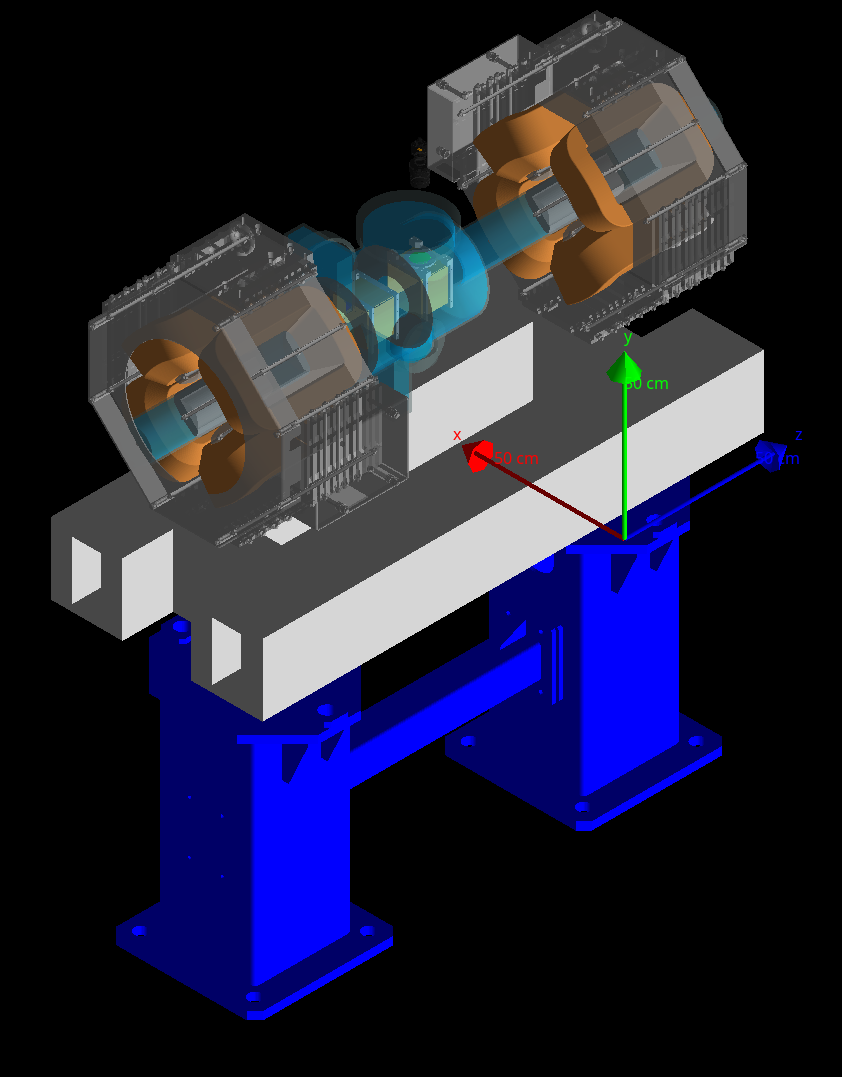
\includegraphics[width=0.5\textwidth]{05_Conclusion/figures/fig000_geant4_sim}
	\caption[The geometry implemented in Geant4]{The geometry implemented in Geant4.}
	\label{chap5:fig:Geant4}
\end{wrapfigure}



\end{refsection}